\documentclass{paper}
\usepackage[T1]{fontenc}
\usepackage{graphicx}
\usepackage[style=numeric, sorting=nty, backend=biber]{biblatex}
\usepackage{url}
\usepackage{hyperref}

\addbibresource{refs.bib}
\graphicspath{{./images}}

\title{Field Programmable Gate Arrays} \author{Viktor Horsmanheimo}

\begin{document}
\maketitle

% introduction
Field programmable gate arrays, or FPGAs have become more and more popular in
the past few decades. So before we begin, what is a field programmable gate
array? Field programmable means that unlike most hardware like normal CPUs, it
can be modified after it's manufactured. So what then is gate array? Gate
arrays are an array of logic gates, they perform simple boolean algebra.
Between the gates we have interconnects, "roads" between the gates which can be
moved to different logic gates. We will go into the specifics of how the logic
gates and interconnects work later.

% history
FPGAs were created in the 1980s by Altera\cite{inthebeginning}, at the time the
logic gates were very large. At the time they didn't have enough logic gates to
actually implement anything useful. They were mostly used to implement
something very simple like handling small inputs from for example a keyboard.
But Moore's law, the law that states that the amount of transistors in a chip
doubles every two years has affected FPGAs as well. This has resulted in that
they have now gotten millions of transistors and have made them powerful enough
to compete with application specific circuits (ASIC).

% compare to ASICs
ASICs are faster than FPGAs. But because ASICs are usually developed one or two
generations back due to it being difficult to always stay on the bleeding edge.
FPGAs have the benefit that they can easily be reprogrammed which means it can
use the latest technology. This means that the they can quite often compete in
terms of speed and power usage of older generation ASICs.

FGPAs have come a long way since then though and are now a critical part of how
modern ASICs are made. They've have made testing ASICs before manufacturing
cheaper \cite{kuon2008fpga} as the manufacturer does not have to build the
physical chip to test it. Instead the chip is emulated fully on the FPGA and
then made sure that it works without errors before creating the ASIC. This
makes the process faster, as making software emulators for hardware can take a
long time.

% optimizations
When FPGAs are used for optimizations in for example cryptography the speed
increases can be quite large. When optimizing polynomial multiplication for
cryptography they saw up to 5 times speed increase compared to application
specific standard products (ASSP)\cite{polynomialmultiplication}. Recently
there has been an increase in use for FPGAs in machine learning
\cite{hardwarecarvision}\cite{mafia} as they provide great parallelization
abilities. For example if you do matrix multiplication on a $100\times 100$
matrix, you could add functionality that it loads all of it and does the
multiplication in one cycle.
\newpage

\begin{figure}[ht]
    \centering
    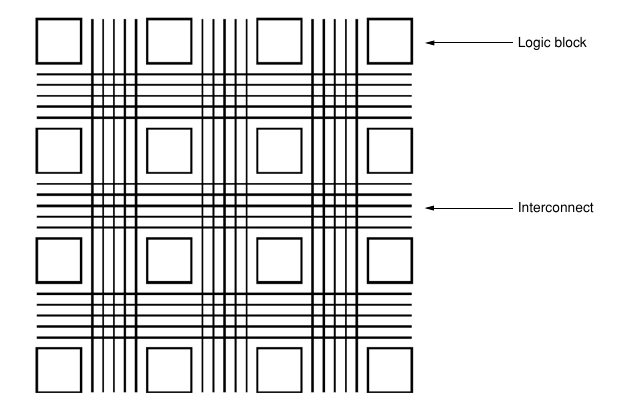
\includegraphics[scale=0.7]{fpga}
    \caption{A simplified picture of an FPGA\cite{reconfSiliconScott}}
    \label{pic:fpga}
\end{figure}

% talk about how they work internally
So how do these chips work internally? There are a couple ways they could be
implemented but as we know, any boolean function can be described using a truth
table. This means that using a lookup table is really efficient, and is what
FPGAs generally use. They are often implemented using $N:1$ multiplexers which
map inputs to an output. Though only using LUTs we cannot store state, so how
is that solved? We can store state using data flip-flops, it can store a single
bit of data. Now we have a full system that can store state and we can actually
implement things in. In \ref{pic:flipflop1} we can see an example
implementation, it uses a multiplexer to get data from either the flip flop or
the LUT. All functions are then broken into small configurable logic
blocks(CLB) containing these LUTs and connected to perform the correct
calculation. This is an example of a LUT we could find in a real
FPGA\cite{reconfSiliconScott}.

\begin{figure}
    \centering
    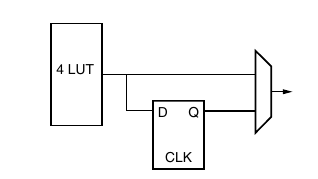
\includegraphics{flipflop}
    \caption{A flip-flop
        combined with a lookup table to store state\cite{reconfSiliconScott}}
    \label{pic:flipflop1}
\end{figure}

Now that we have a picture of how the calculations are done, we'll
now talk about the interconnects and how the data is transferred between the
modules. These interconnects cover the entire chip and is a core feature of how
these reprogrammable chips work in the first place. There are multiple ways
they can be connected and each have both pros and cons. Nearest neighbor is the
simplest one, you connect the modules to the block that is closest.
This isn't optimal as if the signal needs to travel far it has to go through a
lot of blocks. The solution for this though is to have a bunch of control blocks
that choose if the signal goes through the logic block or forwarded to a
switch block that redirects it further. This way the signal doesn't have to
travel through every logic block. These control blocks and switch blocks are
what gives the FPGAs it's reprogrammability.

% ways of configuration TODO
There are a number of different ways the reprogrammability can be implemented.
We'll go into two of the implementations, SRAM based and anti-fuse based.
Essentially FPGAs have two states, configuration-mode, and user-mode, when
configuring the FPGA you send a bit stream through a special set of pins. After
which the FPGA changes to user-mode and runs as configured. More detailed
explanations of how configuration is done dependent on which board you use and
out of scope for this essay. SRAM based FPGAs essentially work by storing the
configuration, which switch blocks lead to where and when a signal should be
sent to a logic block by the control block in static RAM, the downside is that
if power is lost so is the configuration.

Before we go into antifuse systems, antifuses are the opposite of a fuse, it
has a high resistance and doesn't let electricity pass until it gets blown
after which it does let electricity pass. You can use this property to
configure the chip. You blow the antifuses to program the FPGA and make the
electricity to go the way you want it to. Unlike the other ways to program an
FPGA, if you use this, the system can not be reprogrammed as you would need to
replace the antifuse which isn't possible. These are optimal in for example
high radiation environments\cite{fpgaradiation}.

% conclusion
As we've seen, FPGAs can be used in various ways and are critical to both
software and hardware development. In the future I believe they will continue
to increase in popularity and are important to be able to implement quick
hardware optimizations.

\printbibliography

\end{document}
